\section*{Inhaltsverzeichnis}
\label{inhaltsverzeichnis}

\vspace*{0.35em}%
\noindent Workshops am Mittwoch \dotfill \pageref{mittwoch-workshops}

\vspace*{0.35em}%
\noindent Workshops am Donnerstag \dotfill \pageref{donnerstag-workshops}

\vspace*{0.35em}%
\noindent Workshops am Freitag \dotfill \pageref{freitag-workshops}

\vspace*{0.35em}%
\noindent Wegskizze zu den Workshopräumen \dotfill \pageref{karte}

\vspace*{0.35em}%
\noindent Vorträge am Mittwoch \dotfill \pageref{mittwoch}

\vspace*{0.35em}%
\noindent Social Event \dotfill \pageref{social-event}

\vspace*{0.35em}%
\noindent Vorträge am Donnerstag \dotfill \pageref{donnerstag}

\vspace*{0.35em}%
\noindent Vorträge am Freitag \dotfill \pageref{freitag}

\vspace*{0.35em}%
\noindent Impressum \dotfill \pageref{impressum}

\vspace*{0.35em}%
\noindent Gebäudeplan \dotfill \pageref{gebaeudeplan}

\begin{center}
	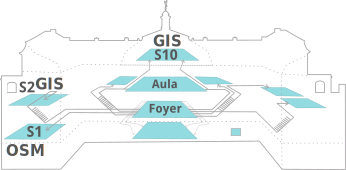
\includegraphics[width=\textwidth]{inhaltsverzeichnis-gebaeudeplan}
\noindent Eine größere Darstellung des Schlosses finden Sie auf Seite \pageref{gebaeudeplan}.
{\small(Bildquelle WWU-Grewer, bearbeitet) }
\end{center}